\subsection{Heuristic generation of the initial solution}

In addition to the randomly generated initial function, I developed the \verb|GenerateHeuristicInitialSolution()|
which construct the initial solution according to an heuristic which aims to minimize the number of constraint violations.

The general outline of the algorithm is as follows:
\begin{enumerate}
  \item Construct a solution by ordering the solution components in an ascending way according to their time windows closing time
  \item For a number of times equal to the solution size divided by 10:
  \begin{enumerate}
    \item Select a random solution component in the solution
    \item Select a neighborhood size randomly.
    \item Shuffle the elements in the chosen neighborhood of the chosen solution
  \end{enumerate}
\end{enumerate}

Due to the lack of time, I was only able to test the heuristic function on a limited number of instances.
The same metrics as in \ref{subsec:metric} will be used to evaluate the algorithms.

\subsubsection{n80w200.001}
\begin{center}
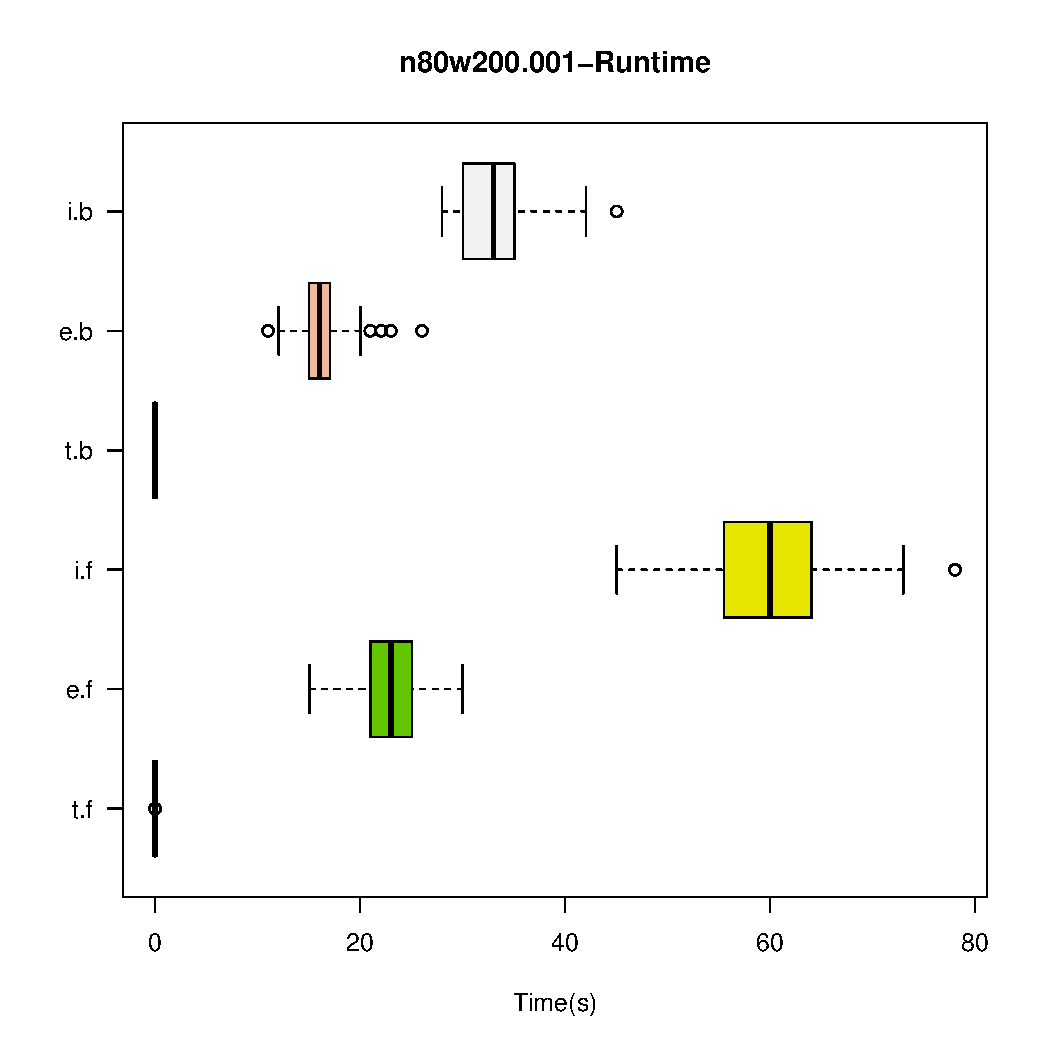
\includegraphics[width=0.6\textwidth,keepaspectratio]{{II-H/n80w200.001-CpuTime}.pdf}
\captionof{figure}{n80w200.001 - Runtime boxplots for the different iterative improvement algorithms with heuristic initialization}
\end{center}

\begin{center}
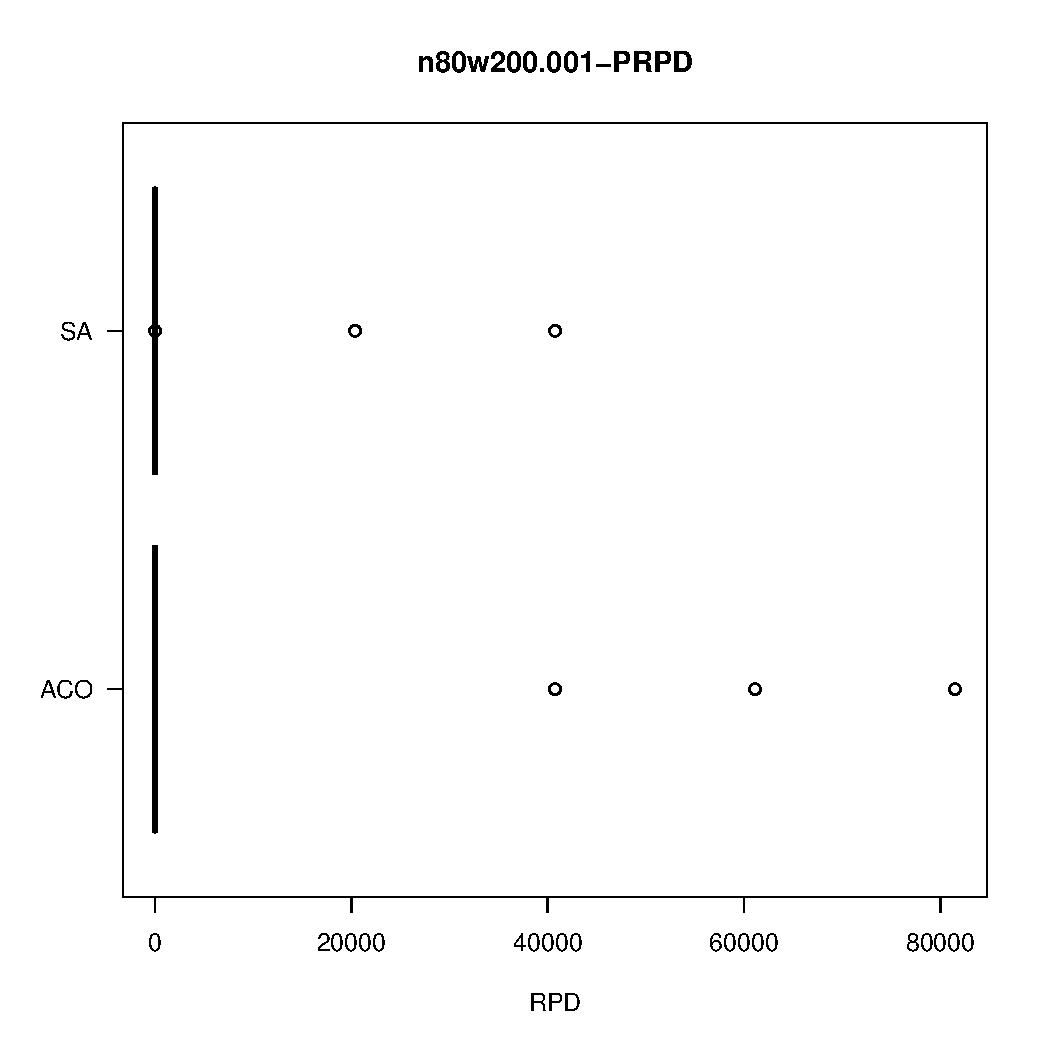
\includegraphics[width=0.6\textwidth,keepaspectratio]{{II-H/n80w200.001-PRPD}.pdf}
\captionof{figure}{n80w200.001 - PRPD boxplots for the different iterative improvement algorithms with heuristic initialization}
\end{center}

\begin{center}
\begin{tabular}{|l|l|}
\hline
\textbf{Test} & \textbf{P-Value} \\
\hline
First vs best - Transpose&3.95591160889952e-18\\
\hline
First vs best - Exchange&3.95591160889952e-18\\
\hline
First vs best - Insert&7.16468868599392e-06\\
\hline
Exchange vs Insert - First&3.95591160889952e-18\\
\hline
Exchange vs Insert - Best&3.9550194074242e-18\\
\hline
\end{tabular}
\captionof{table}{n80w200.001 - Results of Wilcoxon paired signed rank test}
\label{tab:w.21}
\end{center}

\subsubsection{n80w200.002}
\begin{center}
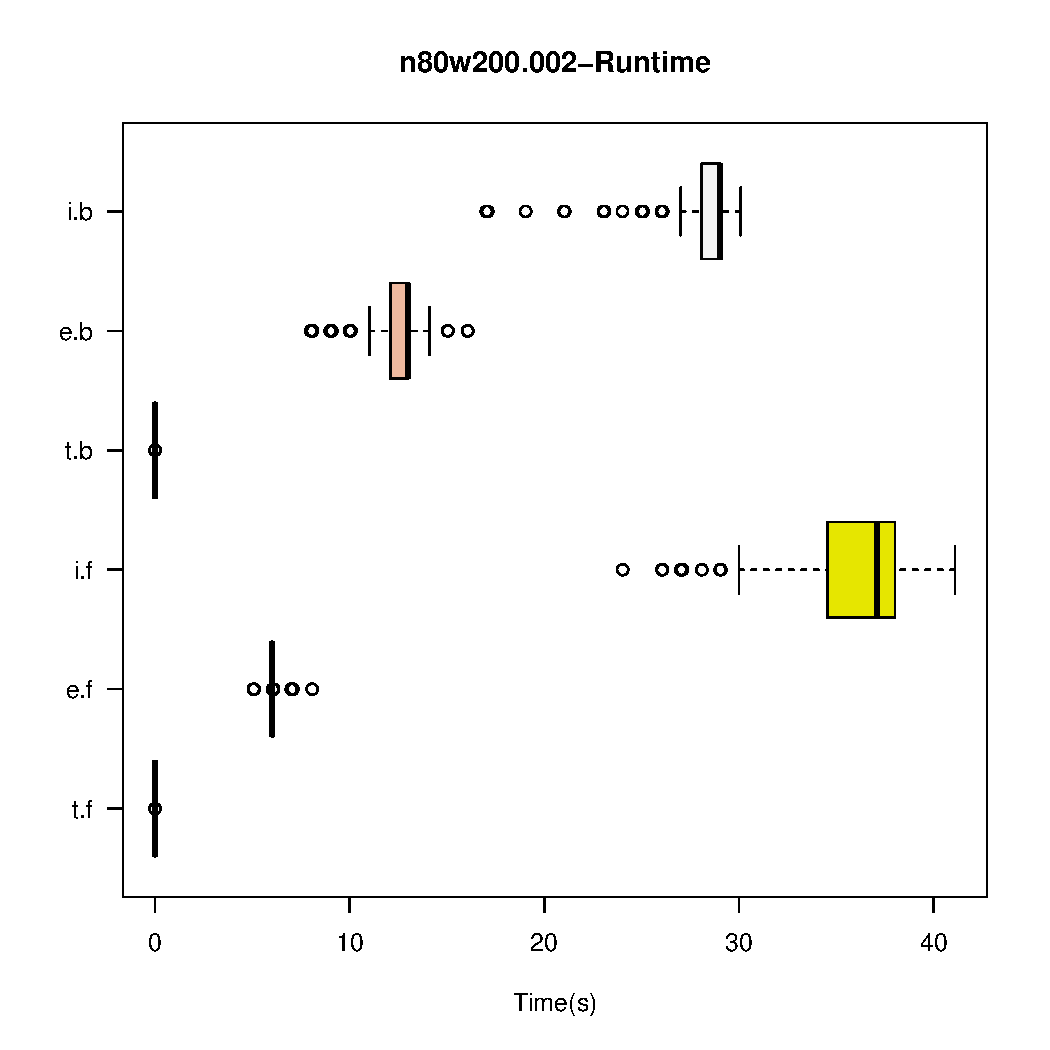
\includegraphics[width=0.6\textwidth,keepaspectratio]{{II-H/n80w200.002-CpuTime}.pdf}
\captionof{figure}{n80w200.002 - Runtime boxplots for the different iterative improvement algorithms with heuristic initialization}
\end{center}

\begin{center}
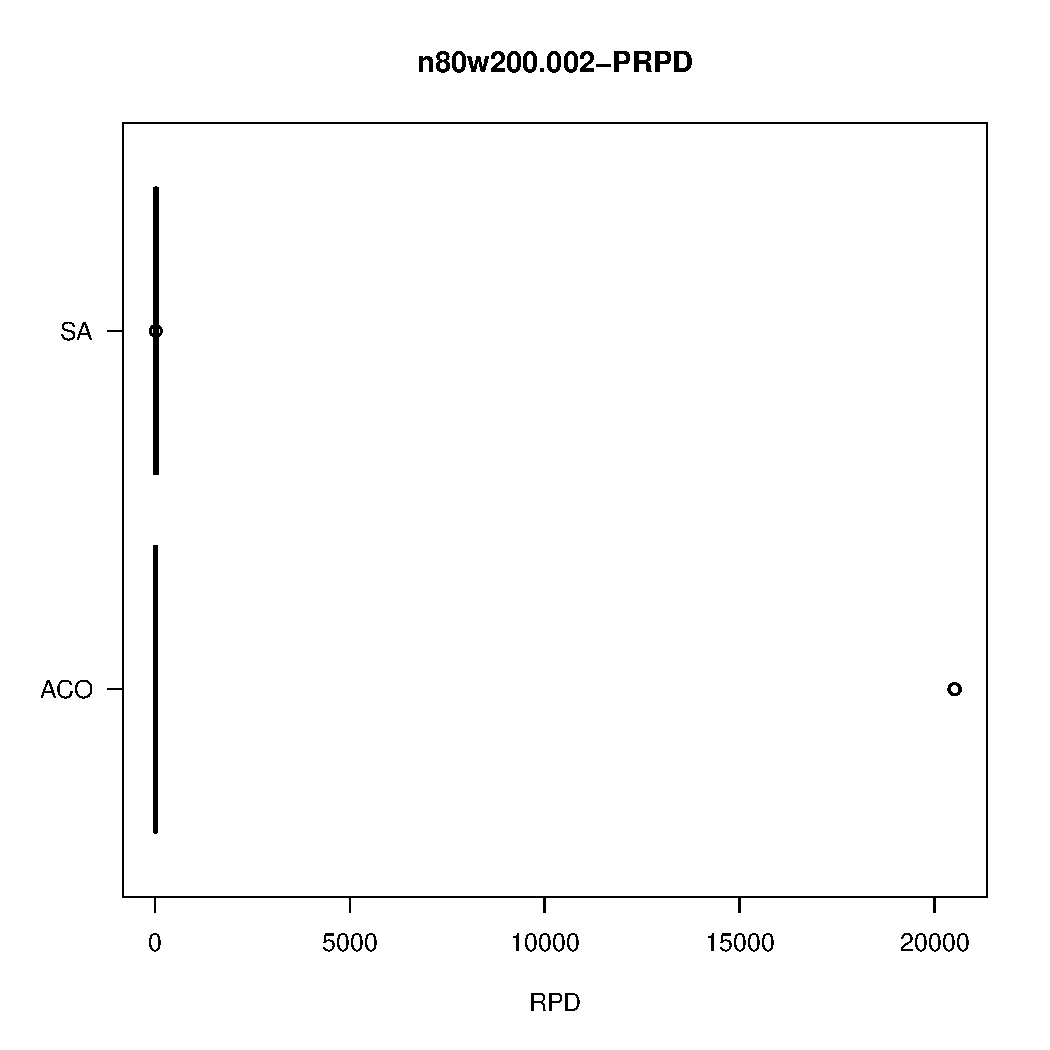
\includegraphics[width=0.6\textwidth,keepaspectratio]{{II-H/n80w200.002-PRPD}.pdf}
\captionof{figure}{n80w200.002 - PRPD boxplots for the different  iterative improvement algorithms with heuristic initialization}
\end{center}

\begin{center}
\begin{tabular}{|l|l|}
\hline
\textbf{Test} & \textbf{P-Value} \\
\hline
First vs best - Transpose&3.95591160889952e-18\\
\hline
First vs best - Exchange&3.95591160889952e-18\\
\hline
First vs best - Insert&1.5011633635878e-17\\
\hline
Exchange vs Insert - First&3.95591160889952e-18\\
\hline
Exchange vs Insert - Best&3.9552424399092e-18\\
\hline
\end{tabular}
\captionof{table}{n80w200.002 - Results of Wilcoxon paired signed rank test}
\label{tab:w.22}
\end{center}

\subsubsection{n80w200.003}
\begin{center}
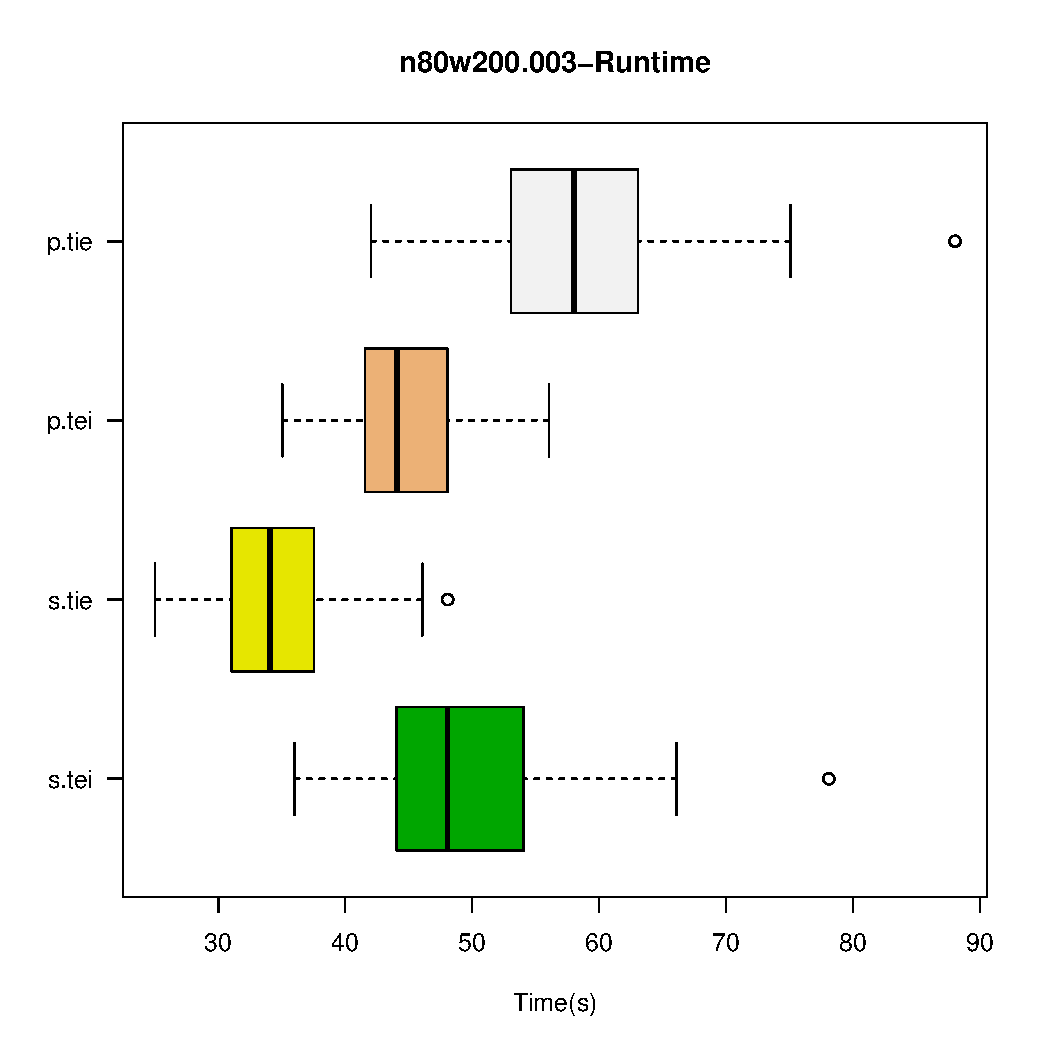
\includegraphics[width=0.6\textwidth,keepaspectratio]{{II-H/n80w200.003-CpuTime}.pdf}
\captionof{figure}{n80w200.003 - Runtime boxplots for the different iterative improvement algorithms with heuristic initialization}
\end{center}

\begin{center}
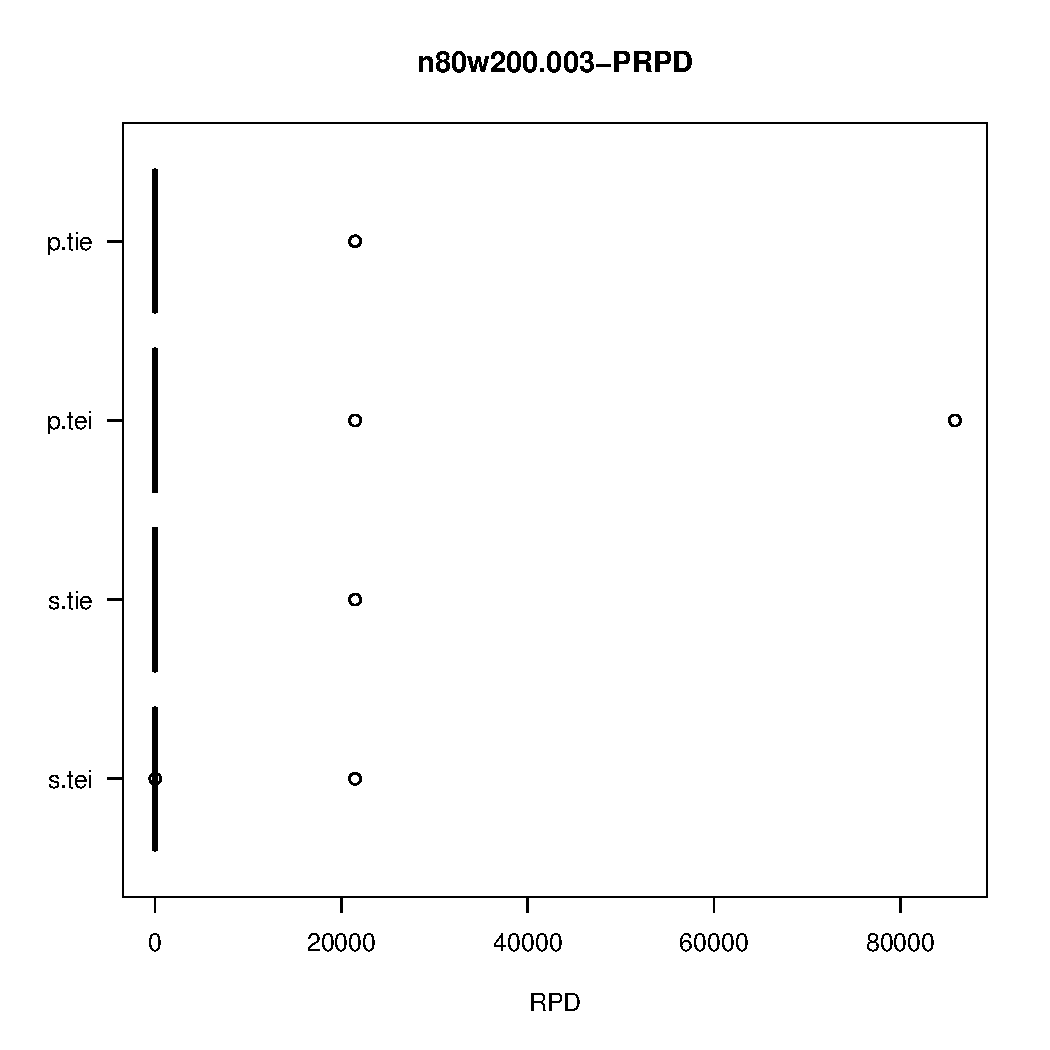
\includegraphics[width=0.6\textwidth,keepaspectratio]{{II-H/n80w200.003-PRPD}.pdf}
\captionof{figure}{n80w200.003 - PRPD boxplots for the different iterative improvement algorithms with heuristic initialization}
\end{center}

\begin{center}
\begin{tabular}{|l|l|}
\hline
\textbf{Test} & \textbf{P-Value} \\
\hline
First vs best - Transpose&3.95591160889952e-18\\
\hline
First vs best - Exchange&3.95591160889952e-18\\
\hline
First vs best - Insert&2.88431649979563e-16\\
\hline
Exchange vs Insert - First&3.9556885406462e-18\\
\hline
Exchange vs Insert - Best&4.33074349739998e-18\\
\hline
\end{tabular}
\captionof{table}{n80w200.003 - Results of Wilcoxon paired signed rank test}
\label{tab:w.23}
\end{center}

\subsection{Statistics}

\subsubsection{Transpose-First Improvement}
\begin{center}
\begin{tabular}{|l|c|l|l|}
\hline
\textbf{Instance}& \textbf{\% Infeasible} & $\mathbf{\bar{PRDP}}$ &$\mathbf{\bar{Runtime}}$\\
\hline
n80w200.003&1&1268365.4&0.0065871265\\
\hline
n80w200.002&1&1071407.7&0.007598828\\
\hline
n80w200.001&1&1243295.2&0.0093113496\\
\hline
\end{tabular}
\captionof{table}{Statistics summary for iterative improvement algorithm with Transpose neighborhood and First Improvement pivoting rule}
\label{tab:t.f.h}
\end{center}

\subsubsection{Transpose-Best Improvement}
\begin{center}
\begin{tabular}{|l|c|l|l|}
\hline
\textbf{Instance}& \textbf{\% Infeasible} & $\mathbf{\bar{PRDP}}$ &$\mathbf{\bar{Runtime}}$\\
\hline
n80w200.003&1&1266853.5&0.0106505552\\
\hline
n80w200.002&1&1071417.8&0.011013054\\
\hline
n80w200.001&1&1240638.1&0.013889943\\
\hline
\end{tabular}
\captionof{table}{Statistics summary for iterative improvement algorithm with Transpose neighborhood and Best Improvement pivoting rule}
\label{tab:t.b.h}
\end{center}

\subsubsection{Exchange-First Improvement}
\begin{center}
\begin{tabular}{|l|c|l|l|}
\hline
\textbf{Instance}& \textbf{\% Infeasible} & $\mathbf{\bar{PRDP}}$ &$\mathbf{\bar{Runtime}}$\\
\hline
n80w200.003&0&27.068636&6.0144574\\
\hline
n80w200.002&0.02&432.979367&6.1109123\\
\hline
n80w200.001&0.87&18146.162472&8.842327\\
\hline
\end{tabular}
\captionof{table}{Statistics summary for iterative improvement algorithm with Exchange neighborhood and First Improvement pivoting rule}
\label{tab:e.f.h}
\end{center}

\subsubsection{Exchange-Best Improvement}
\begin{center}
\begin{tabular}{|l|c|l|l|}
\hline
\textbf{Instance}& \textbf{\% Infeasible} & $\mathbf{\bar{PRDP}}$ &$\mathbf{\bar{Runtime}}$\\
\hline
n80w200.003&1&180715.273&17.098637\\
\hline
n80w200.002&1&92647.622&12.3893899\\
\hline
n80w200.001&1&694332.77&17.575257\\
\hline
\end{tabular}
\captionof{table}{Statistics summary for iterative improvement algorithm with Exchange neighborhood and Best Improvement pivoting rule}
\label{tab:e.b.h}
\end{center}

\subsubsection{Insert-First Improvement}
\begin{center}
\begin{tabular}{|l|c|l|l|}
\hline
\textbf{Instance}& \textbf{\% Infeasible} & $\mathbf{\bar{PRDP}}$ &$\mathbf{\bar{Runtime}}$\\
\hline
n80w200.003&0.03&2587.6121429&30.841123\\
\hline
n80w200.002&0&9.9979528&35.672697\\
\hline
n80w200.001&0.1&4897.5213208&32.775532\\
\hline
\end{tabular}
\captionof{table}{Statistics summary for iterative improvement algorithm with Insert neighborhood and First Improvement pivoting rule}
\label{tab:i.f.h}
\end{center}

\subsubsection{Insert-Best Improvement}
\begin{center}
\begin{tabular}{|l|c|l|l|}
\hline
n80w200.003&0&4.3454898&23.452399\\
\hline
n80w200.002&0.01&630.9635938&27.922795\\
\hline
n80w200.001&0.1&3680.5235577&32.277408\\
\hline
\end{tabular}
\captionof{table}{Statistics summary for iterative improvement algorithm with Insert neighborhood and Best Improvement pivoting rule}
\label{tab:i.b.h}
\end{center}

\subsection{Results discussion}
By looking at tables \ref{tab:t.f.h}, \ref{tab:t.b.h}, \ref{tab:e.f.h}, \ref{tab:e.b.h} \ref{tab:i.f.h}, \ref{tab:i.b.h} on can see that:
\begin{itemize}

\item The only neighborhood type which does not allow to generate feasible solution is the Transpose one.

\item By using the heuristic, also the algorithm using the Exchange neighbohood is able to generate feasible solutions that are close to the best known value.

\item The use of the heuristic allows for a consistent reduction of the runtime, which becomes on average on half ot the runtime of the algorithm with random initiaalisation on the same instances.

\item The solution quality of the generated solutions also benefits from the introduction of an heurstic initialization.

\item Tables \ref{tab:w.21}, \ref{tab:w.22}, \ref{tab:w.23} contain, in any case, p-values considerably smaller than the significance level ($\alpha=0.05$). 

This implies that the null hypothesis corresponding to the equality of the median values of the differences of the two distributions can be rejected, hence assessing the existence of a statistically significant difference among the solution quality generated by analyzed algorithms.


\end{itemize}
